\documentclass[letterpaper]{article}
\usepackage{url,graphicx,tabularx,array,amsmath,amssymb,amsthm,bbm,textcomp,algorithm}
\usepackage[noend]{algpseudocode}
\usepackage{aaai} 
\usepackage{times} 
\usepackage{helvet} 
\usepackage{courier} 
\setlength{\pdfpagewidth}{8.5in} 
\setlength{\pdfpageheight}{11in}


\newcommand{\unionf}{\bigcup_{n=1}^{\infty} \mathcal{F}_n}
\newcommand{\F}{\mathcal{F}}
\newcommand{\E}{\mathbb{E}}
\newcommand{\PP}{\mathbb{P}}
\newcommand{\Hi}{\mathcal{H}}
\newcommand{\A}{\mathcal{A}}
\newcommand{\Aseq}{\{A_k\}_{k=1}^{\infty}}
\newcommand{\unionA}{\bigcup_{k=1}^{\infty} A_k}
\newcommand{\argmax}{\operatornamewithlimits{argmax}}

\newenvironment{dedication}
        {\vspace{0.0ex}\begin{quotation}\begin{center}\begin{em}}
        {\par\end{em}\end{center}\end{quotation}}

\makeatletter
\def\BState{\State\hskip-\ALG@thistlm}
\makeatother

\pdfinfo{
/Title (Inertial Hidden Markov Models: Modeling Change in Multivariate Time Series)
/Author (George D. Montanez, Saeed Amizadeh, Nikolay Laptev)
/Keywords (segmenting time series, unsupervised learning, hidden Markov models, state persistence, inertial HMM)
}

\title{Inertial Hidden Markov Models: Modeling Change in Multivariate Time Series}

%...............................................................................
%                                   Authors
%...............................................................................

\author{George D. Monta\~nez \\
School of Computer Science\\
Carnegie Mellon University\\
Pittsburgh, PA USA\\
\texttt{gmontane@cs.cmu.edu} \\
\And
Saeed Amizadeh\\
Yahoo Labs\\
Sunnyvale, CA USA\\
\texttt{amizadeh@yahoo-inc.com}\\
\And
Nikolay Laptev\\
Yahoo Labs\\
Sunnyvale, CA USA\\
\texttt{nlaptev@yahoo-inc.com}}

\begin{document}

\maketitle

\begin{abstract}
    Faced with the problem of characterizing systematic changes in multivariate
    time series in an unsupervised manner, we derive and test two methods of regularizing hidden
    Markov models for this task. Regularization on state transitions provide
    smooth transitioning among states, such that the sequences are split into
    broad, contiguous segments. Our methods are compared with a recent
    hierarchical Dirichlet process hidden Markov model (HDP-HMM) and a baseline
    standard hidden Markov model, of which the former suffers from poor
    performance on moderate-dimensional data and sensitivity to parameter
    settings, while the latter suffers from rapid state transitioning,
    over-segmentation and poor performance on a segmentation task involving
    human activity accelerometer data from the UCI Repository.
    The regularized methods developed here are able to perfectly characterize
    change of behavior the human activity data in roughly half of the real-data
    test cases, with accuracy of 94\% and low variation of information. In contrast to the
    HDP-HMM, our methods provide simple, drop-in replacements for standard
    hidden Markov model update rules, allowing standard expectation maximization
    (EM) algorithms to be used for learning. 
%     Lastly, we make progress towards
%     tuning the regularization strength in an unsupervised manner and derive
%     equations for online learning of the regularized HMM parameters.
\end{abstract}

\section{Introduction}
\begin{dedication} ``Some seek complex solutions to simple problems; it is better to find simple solutions to complex problems.'' - \emph{Soramichi Akiyama}
\end{dedication}

Time series data arise in different areas of science and technology, describing
the behavior of both natural and man-made systems over time. These
behaviors are often quite complex with uncertainty, which in turn require us to
incorporate sophisticated dynamics and stochastic models to model them.
Furthermore, these complex behaviors can \emph{change} over time due to some external event and/or some internal
systematic change of dynamics/distribution. For example, consider the case of
monitoring one's physical activity via an array of accelerometer body sensors
over time. A certain pattern emerges on the time series of the sensors' readings
while the person is walking; however, this pattern quickly changes to a new one
as the person starts running. From the data analysis perspective, it is
important to first detect these \emph{change points} as they are quite often
indicative of an ``interesting'' event or an anomaly in the system. We
are also interested in characterizing the new \emph{state} of the system (e.g. running vs.\
walking) which reflects its modus operandi. Change point detection methods~\cite{} have been proposed
to answer the first question while the classical Hidden Markov Models (HMM) can
answer both.

One crucial observation in many real-world systems (natural and man-made),
however, is that the behavior changes are typically infrequent; that is, the
system takes some (unknown) time before it changes its behavior to a new modus operandi. For
instance, in our earlier example, it is unlikely that a person changes between
walking and running very frequently, making the durations of different
activities over time relatively long and highly variable. We refer to this as the
\emph{inertial property}, alluding to the physical property of matter that
ensures it will continue along a fixed course unless acted upon by an external
force. Unfortunately, the classical HMMs are not equipped with sufficient
mechanisms to capture this property and quite often result in a high rate of
state transitioning and subsequently false positives in terms of detecting
change points.

Few solutions exist in the literature to address this problem. In
the context of Markov models, Fox \emph{et al.}~\cite{fox2011sticky}\ have
recently proposed the \emph{sticky hierarchical Dirichlet process hidden Markov
model (HDP-HMM)} which uses a Bayesian non-parametric approach with appropriate
priors to promote self-transitioning (or \emph{stickiness}) for HMMs. Despite its
nice theoretical foundations, the HDP-HMM is not a practical solution in many real-world situations.
In particular, the performance of the HDP-HMM tends to degrade as the
dimensionality of the problem increases beyond ten dimensions. Moreover, due to 
iterative Gibbs sampling for its learning, the HDP-HMM can become computationally prohibitive. 
In practice, the most significant drawback of the HDP-HMM originates with its non-parametric 
Bayesian nature: due to the existence of many hyperparameters, the search space for initial tuning is 
exponentially large which significantly affects the learning quality for a given task.

In this paper, we propose a regularization-based framework for HMMs, called
\emph{Inertial hidden Markov models} (Inertial HMMs), which are biased towards the inertial 
state-transition property. Similar to the HDP-HMM, our framework is based on 
theoretically sound foundations, yet much simpler and more intuitive than the HDP-HMM. 
In particular, our framework has only two initial parameters for which we have 
developed intuitive initialization techniques that significantly minimize the effort 
needed for parameter tuning. Furthermore, as we show later, our proposed
methods in practice boil down to upgraded update rules for standard HMMs. This allows one to easily 
upgrade existing HMM libraries to take advantage of our methods, while still preserving the
computational efficiency of the standard HMM approach. By performing rigorous
experiments on both synthetic and moderate dimensional real datasets, we show
that Inertial HMMs are not only much faster than the HDP-HMM, but also produce 
significantly better detection, suggesting Inertial HMMs as a far more practical 
choice in comparison to the current state-of-the-art.

\section{Problem Statement}

Let $\mathbf{X} = \{\mathbf{x}_1, \ldots, \mathbf{x}_T\}$ denote a
$d$-dimensional multivariate time series, where $\mathbf{x}_t \in \mathbb{R}^d$.
Given such a time series, we seek to segment $\mathbf{X}$ along the time axis
into \emph{segments}, where each segment corresponds to a subsequence
$\mathbf{X}_{i\ldots i+m} = \{\mathbf{x}_i, \ldots, \mathbf{x}_{i+m}\}$ and maps
to a predictive (latent) state $\mathbf{z}$, represented as a one-of-$K$ vector,
where $|\mathbf{z}| = K$ and $\sum_{i=1}^{K}z_{t,i} = 1$. For simplicity of
notation, let $\mathbf{z}_{t} = k$ denote $z_{t,k} = 1$ and let $\mathbf{Z} =
\{\mathbf{z}_1, \ldots, \mathbf{z}_T\}$ denote the sequence of latent states.
Then for all $\mathbf{x}_{t}$ mapping to state $k$, we require that
\begin{align*}
    \Pr(\mathbf{x}_{t+1}|\mathbf{X}_{1\ldots t}, \mathbf{z}_t = k) 
    &= \Pr(\mathbf{x}_{t+1}| \mathbf{z}_t = k) \\
    &= \Pr(\mathbf{x}_{t'+1}| \mathbf{z}_{t'} = k) \\
    &= \Pr(\mathbf{x}_{t'+1}| \mathbf{X}_{1\ldots t'}, \mathbf{z}_{t'} = k).
\end{align*}
Thus, the conditional distribution over futures at time $t$ conditioned on being
in state $k$ is equal to the distribution over futures at time $t'$ conditioned
on being in the same state. Thus, we assume conditional independence given
state, and stationarity of the generative process.

We impose two additional criteria on our models. First, we seek models
with a small number of latent states, $K \ll T$, and second, we desire state
transition sequences with the inertial property, as defined previously, where 
the transitioning of states does not occur too rapidly. 

The above desiderata must be externally imposed on our model, since simply
maximizing the likelihood of the data will result in $K = T$ (i.e., each sample
corresponds a unique state/distribution), and in general we may have rapid
transitions among states. For the first desideratum,  we choose the number of
states in advance as is typically done for hidden Markov
models~\cite{rabiner1989tutorial}. For the second, we directly alter the
probabilistic form of our model to include a parameterized regularization that
reduces the likelihood of transitioning between different latent states.

%\subsection{Problem Input and Output}
%
%As stated above, we are given a single $d$-dimensional multivariate time series of $T$ time samples. Alternatively, the single time series can be thought of as a collection of $d$ one-dimensional time series. As the generative story, we assume that at each time step $t$ a state $\mathbf{z}_t$ is chosen, given the previous state $\mathbf{z}_{t-1}$, according to the transition probabilities governing states. A $d$-dimensional point-sample is then drawn according to the emission density for state $\mathbf{z}_t$, and the process repeats for $1 < t \leq T$.
%
%The output of the process is a list of integer tuples $(t, k)$, where $1 \leq t \leq T$ denotes the ending time of the segment and $1 \leq k \leq K$ the state that occurs during that segment. 

\section{Inertial Hidden Markov Models}

Hidden Markov models (HMMs) are a class of long-studied probabilistic models
well-suited for sequential data~\cite{rabiner1989tutorial}. As a starting point
for developing our inertial HMMs, we begin a standard $K$-state HMM with
Gaussian emission densities. HMMs (locally) maximize the likelihood of the data,
but typically do not guarantee slow inertial transitioning among states. The
number of states must be specified in advance, but no other parameters need to
be given, as the remaining parameters are all estimated directly from the
data.

To accommodate the inertial transition requirement, we derive two different
methods of enforcing state-persistence in HMMs. Both methods alter the
probabilistic form of the complete data joint likelihood, which result
in altered transition matrix update equations. The resulting update equations
share a related mathematical structure and, as is shown in
the Experiments section, have similar performance in practice.

We will next describe both methods and provide outlines of their derivations. 
% (the pseudo-observation inertial HMM).

\subsection{Maximum A Posteriori (MAP) Regularized HMM}

Following~\cite{MAP1994}, we alter the standard HMM to include a Dirichlet prior on the transition probability matrix, such that transitions out-of-state are penalized by some regularization factor. A Dirichlet prior on the transition matrix $\mathbf{A}$, for the $j$th row, has the form
\begin{align*}
    p(A_j; \eta) &\propto \prod_{i=1}^{K} A_{jk}^{\eta_{jk}-1}
\end{align*}
where the $\eta_{jk}$ are free parameters and $A_{jk}$ is the transition probability from state $j$ to state $k$. The posterior joint density over $\mathbf{X}$ and $\mathbf{Z}$ becomes
\begin{align*}
    P(\mathbf{X}, \mathbf{Z} ; \mathbf{\theta}, \eta) 
    &\propto \left[\prod_{i=1}^{K}\prod_{i=1}^{K} A_{jk}^{\eta_{jk} - 1}\right] P(\mathbf{X}, \mathbf{Z} \mid \mathbf{A}; \mathbf{\theta}) 
\end{align*}
and the log-likelihood is
\begin{align*}
\ell(\mathbf{X}, \mathbf{Z} ; \mathbf{\theta}, \eta) 
&\propto \sum_{i=1}^{K}\sum_{i=1}^{K} (\eta_{jk} - 1)\log A_{jk} + \log P(\mathbf{z}_{1}; \theta) \\
&+ \sum_{t=1}^{T}\log P(\mathbf{x}_t|\mathbf{z}_t; \mathbf{\theta}) + \sum_{t=2}^{T}\log P(\mathbf{z}_t|\mathbf{z}_{t-1}; \mathbf{\theta}).
\end{align*}

MAP estimation is then used in the M-step of the EM algorithm, to update the transition probability matrix. Maximizing, with appropriate Lagrange multiplier constraints, we obtain the update equation for the transition matrix, 
\begin{align}
    A_{jk} &= \frac{(\eta_{jk} - 1) + \sum_{t=2}^{T} \xi(z_{(t-1)j}, z_{tk})}   
    {\sum_{i=1}^{K}(\eta_{ji} - 1) + \sum_{i=1}^{K}\sum_{t=2}^{T} \xi(z_{(t-1)j}, z_{ti})}.
\end{align}
where the $\xi(z_{(t-1)j}, z_{tk})=\mathbb{E}[z_{(t-1)j}z_{tk}]$.

Given our prior, we can control the probability of self-transitions among states, but this method requires that we choose a set of $K^2$ parameters for the Dirichlet prior. However, since we are solely concerned about increasing the probability of self-transitions, we can reduce these parameters to a single parameter $\lambda$ governing the amplification of self-transitions. We therefore define $\eta_{jk} = 1$ when $j\not=k$ and $\eta_{kk}= \lambda \geq 1$ otherwise, and the transition update equation becomes
\begin{align}\label{eq:MAP-final}
    A_{jk} &= \frac{(\lambda - 1){\mathbbm{1}(j = k)} + \sum_{t=2}^{T} \xi(z_{(t-1)j}, z_{tk})}   
    {(\lambda - 1) + \sum_{i=1}^{K}\sum_{t=2}^{T} \xi(z_{(t-1)j}, z_{ti})}
\end{align}
where $\mathbbm{1}(\cdot)$ denotes the indicator function.

\subsection{Inertial Regularization via Pseudo-observations}

Alternatively, we can alter the HMM likelihood function to include a latent binary random variable,
$V$, indicating that a self-transition was chosen at random from among all transitions, according to some distribution. 
Thus, we view the transitions as being partitioned into two sets, self-transitions and non-self-transitions, and
we draw a member of the self-transition set according to a Bernoulli
distribution governed by parameter $p$. Given a latent state sequence
$\mathbf{Z}$, with transitions chosen according to transition matrix
$\mathbf{A}$, we define $p$ as a function of both $\mathbf{Z}$ and $\mathbf{A}$.
We would like $p$ to have two properties: 1) it should increase with increasing
$\sum_k A_{kk}$ (probability of self-transitions) and 2) it should increase as
the number of self-transitions in $\mathbf{Z}$ increases. This will allow us to
encourage self-transitions as a simple consequence of maximizing the likelihood
of our observations.

We begin with a version of $p$ based on a penalization constant $0 < \epsilon <
1$ that scales appropriately with the number of self-transitions. If we raise
$\epsilon$ to a large positive power, the resulting $p$ will decrease. Thus, we
define $p$ as $\epsilon$ raised to the number of non-self-transitions, $M$, in
the state transition sequence, so that the probability of selecting a
self-transition increases as $M$ decreases. Using
the fact that $M=(T-1) - \sum^{T}_{t=2}\sum^{K}_{k=1}z_{(t-1)k}z_{tk}$, we obtain
\begin{align}
    p &= \epsilon^M = \epsilon^{\sum^{T}_{t=2}1 -
    \sum^{T}_{t=2}\sum^{K}_{k=1}z_{(t-1)k}z_{tk}} \notag\\
      &= \epsilon^{\sum^{T}_{t=2}\sum^{K}_{k=1}z_{(t-1)k} - \sum^{T}_{t=2}\sum^{K}_{k=1}z_{(t-1)k}z_{tk}} \notag\\
      &= \prod^{T}_{t=2}\prod_{k=1}^{K}\epsilon^{z_{(t-1)k} - z_{(t-1)k}z_{tk}}. \label{eq:eps-0}
\end{align}

Since $\epsilon$ is arbitrary, we choose $\epsilon = A_{kk}$, to allow $p$ to scale appropriately with increasing probability of self-transition. We therefore arrive at
\begin{align*}
    p &= \prod^{T}_{t=2}\prod^{K}_{k=1}A_{kk}^{z_{(t-1)k} - z_{(t-1)k}z_{tk}}.
\end{align*}
Thus, we define $p$ as a computable function of $\mathbf{Z}$ and $\mathbf{A}$.
Defining $p$ in this deterministic manner is equivalent to choosing the
parameter value from a degenerate probability distribution that places a single
point mass at the value computed, allowing us to easily obtain a posterior
distribution on $V$. Furthermore, we see that the function increases as the
number of self-transitions increases, since $A_{kk} \leq 1$ for all $k$, and $p$
will generally increase as $\sum_k A_{kk}$ increases. Thus, we obtain a
parameter $p \in (0,1]$ that satisfies all our desiderata.
With $p$ in hand, we say that $V$ is drawn according to the Bernoulli
distribution, Bern($p$), and we observe $V = 1$ (i.e., a member of the
self-transition set was chosen). 
% Since $P(V = 1|\mathbf{Z};\mathbf{A}) = p$, we
% have
% \begin{align*}
%     P(V = 1|\mathbf{Z}; \mathbf{A}) &= \prod^{T}_{t=2}\prod^{K}_{k=1}A_{kk}^{z_{(t-1)k} - z_{(t-1)k}z_{tk}}.
% \end{align*}
To gain greater control over the strength of regularization, let $\lambda$ be a
positive integer and $\mathbf{V}$ be an $\lambda$-length sequence of
pseudo-observations, drawn i.i.d.\ according to Bern($p$). Since $P(V =
1|\mathbf{Z};\mathbf{A}) = p$, we have
\begin{align*}
    P(\mathbf{V} = \mathbf{1}|\mathbf{Z}; \mathbf{A}) &= \left[\prod^{T}_{t=2}\prod^{K}_{k=1}A_{kk}^{z_{(t-1)k} - z_{(t-1)k}z_{tk}}\right]^\lambda
\end{align*}
where $\mathbf{1}$ denotes the all-ones sequence of length $\lambda$.

Noting that $\mathbf{V}$ is conditionally independent of $\mathbf{X}$ given the
latent state sequence $\mathbf{Z}$, we maximize (with respect to $A_{jk}$) the expected 
(with respect to $\mathbf{Z}$) joint log-density over $\mathbf{X}$, $\mathbf{V}$, and $\mathbf{Z}$ parameterized by
$\mathbf{\theta} = \{\mathbf{\pi},\mathbf{A}, \mathbf{\phi}\}$, which are the start-state
probabilities, state transition matrix and emission parameters, respectively. Using appropriate Lagrange multipliers, we obtain the regularized
maximum likelihood estimate for $A_{jk}$:
\begin{align}\label{eq:PSO-final}
    A_{jk} &= \frac{B_{j,k,T} + {\mathbbm{1}(j = k)}C_{j,k,T}} 
                   {\sum_{i=1}^{K} B_{j,i,T} + C_{j,j,T}}
\end{align}
where $\mathbbm{1}(\cdot)$ denotes the indicator function, $\gamma(z_{tk}) = \mathbb{E}[z_{tk}]$ and
\begin{align}\label{eq:PSO-final-C-part}
    B_{j,k,T} &= \sum_{t=2}^{T} \xi(z_{(t-1)j}, z_{tk}), \notag\\
    C_{j,k,T} &= \lambda\left[\sum_{t=2}^{T}[\gamma(z_{(t-1)k}) - \xi(z_{(t-1)j}, z_{tk})]\right].
\end{align}
The forward-backward algorithm can then be used for efficient computation of the $\gamma$ and $\xi$ values, as in standard HMMs~\cite{bishop2007pattern}.

Ignoring normalization, we see that
\begin{align*}
    A_{jk} &\propto \begin{cases} 
                B_{j,k,T} + C_{j,j,T} & \mbox{if } j=k \\ 
                B_{j,k,T} & \mbox{otherwise.}
              \end{cases}
\end{align*}
Examining the $C_{j,j,T}$ term (i.e., Equation~(\ref{eq:PSO-final-C-part})), we see that $\lambda$ is a multiplier of
additional mass contributions for self-transitions, where the contributions are
the difference between $\gamma(z_{(t-1)j})$ and $\xi(z_{(t-1)j}, z_{tj})$. These
two quantities represent, respectively, the expectation of being in a state $j$
at time $t-1$ and the expectation of remaining there in the next time step. The
larger $\lambda$ or the larger the difference between arriving at a state and
remaining there, the greater the additional mass given to self-transition.

\subsubsection{Scale-Free Regularization}

In Equation~\ref{eq:MAP-final}, the strength of the regularization diminishes
with growing $T$, so that asymptotically the regularized estimate and
unregularized estimate become equivalent. While this is desirable in many
contexts, maintaining a consistent strength of inertial regularization becomes
important with time series of increasing length, as is the case with online
learning methods. Figure~\ref{fig:short-real-data} shows a regularized
segmentation of human accelerometer data (discussed later in the Experiments
section), where the regularization is strong enough to correctly segment the
series into large, contiguous sections. If we then increase the number of data
points in each section by a factor of ten while keeping the same regularization
parameter setting, we see that the regularization is no longer strong enough, as
is shown in Figure~\ref{fig:long-real-data}. Two of the sections have become
splintered into small, choppy regions. Thus, the $\lambda$ parameter is
sensitive to the size of the time series.
\begin{figure}[htbp]
  \centering
    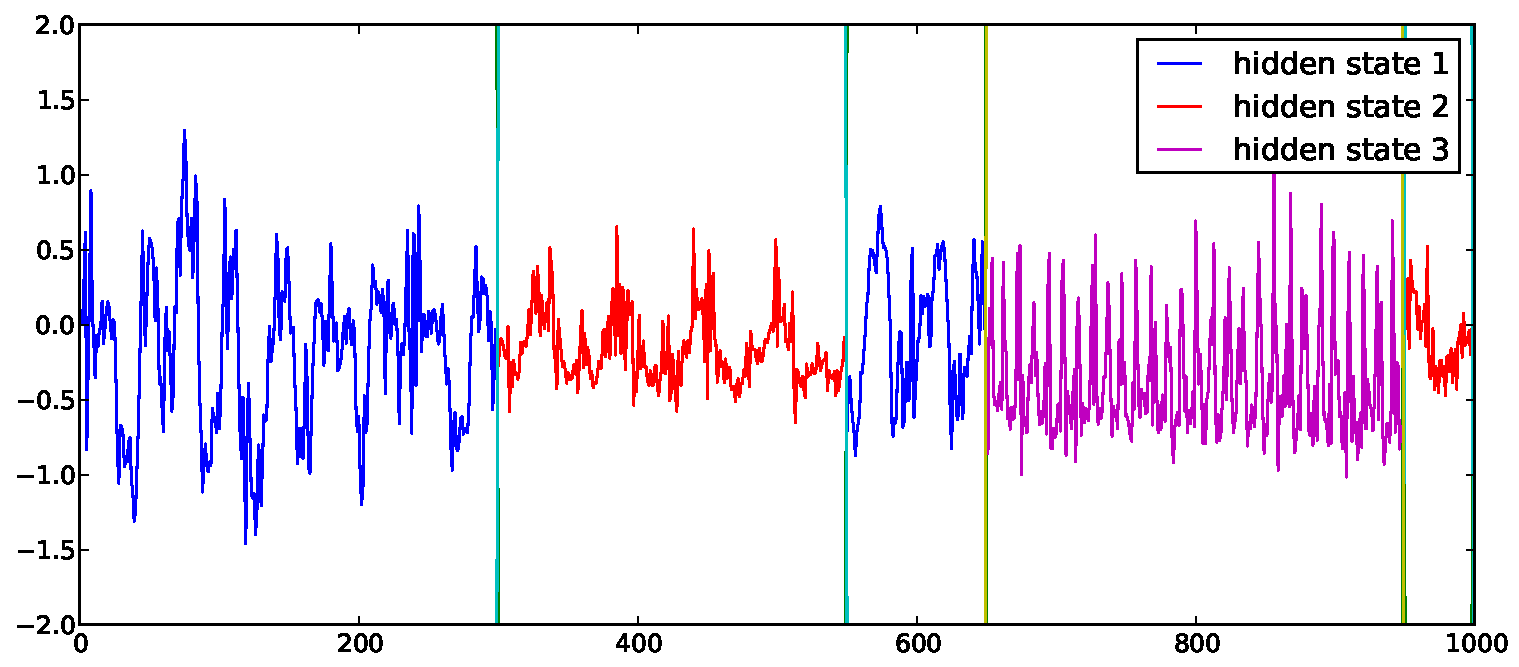
\includegraphics[width=0.8\linewidth]{images/MAP_results_hard_activity_short_3_states.pdf}
  \caption{\small{Human activities accelerometer data, short sequence. Vertical
  partitions correspond to changes of state.}}
  \label{fig:short-real-data}  
\end{figure}

\begin{figure}[htbp]
  \centering
    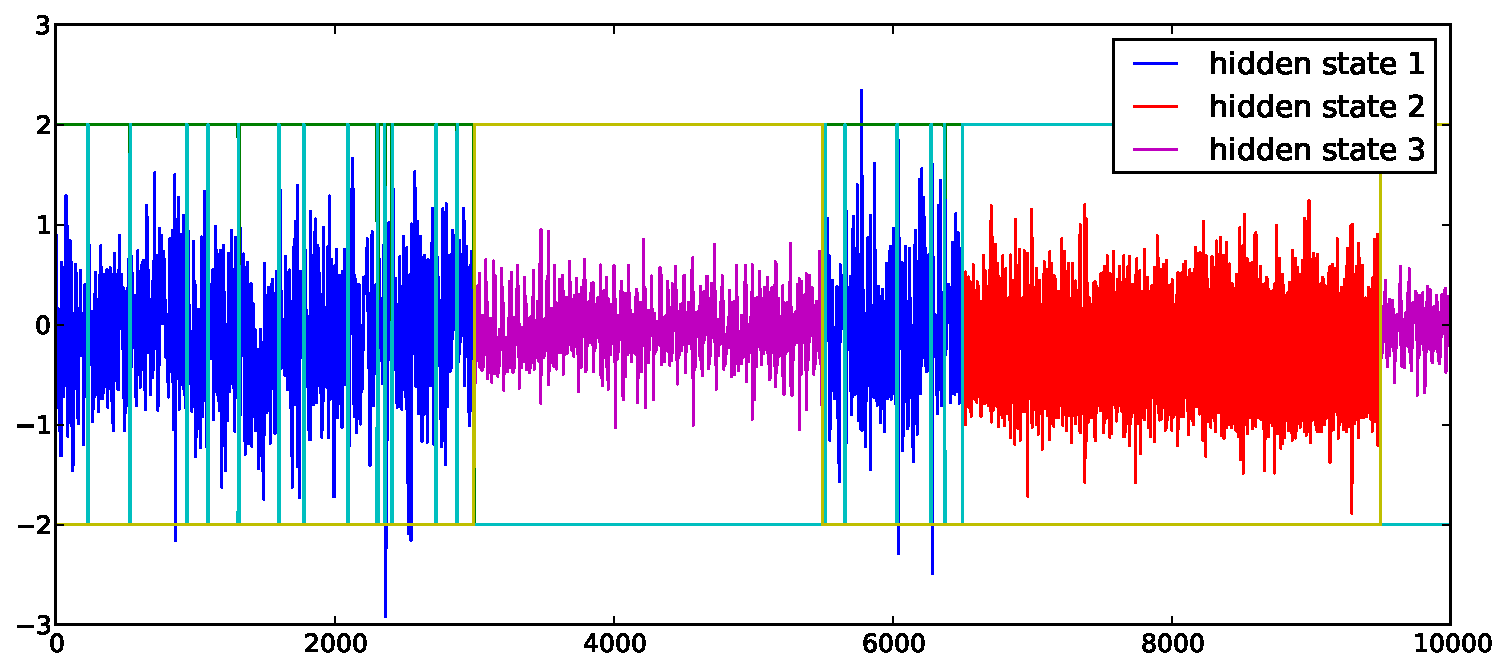
\includegraphics[width=0.8\linewidth]{images/MAP_results_hard_activity_long_3_states.pdf}    
  \caption{\small{The long sequence human activities accelerometer data using
  regularization parameter from short sequence.}}
  \label{fig:long-real-data}
\end{figure}

We desire models where the regularization strength is scale-free, having roughly the same strength regardless of how the time series grows. To achieve this, we define the $\lambda$ parameter to scale with the number of transitions, namely $\lambda = (T-1)^\zeta$, and our scale-free update equation becomes
\begin{align}\label{eq:SCALE-FREE-MAP}
    A_{jk} &= \frac{((T - 1)^{\zeta}-1){\mathbbm{1}(j = k)} + \sum_{t=2}^{T} \xi(z_{(t-1)j}, z_{tk})}   
    {((T - 1)^{\zeta} - 1) + \sum_{i=1}^{K}\sum_{t=2}^{T} \xi(z_{(t-1)j}, z_{ti})}.
\end{align}
This preserves the effect of regularization as $T$ increases, and $\zeta$
becomes our new regularization parameter, controlling the strength of the
regularization. For consistency, we also re-parameterize
Equation~(\ref{eq:PSO-final-C-part}) using $\lambda = (T-1)^\zeta$.

\subsubsection{Towards Parameter-Free Regularization}\label{sec:param-free}

Although our methods require specifying the strength of regularization in advance, one can avoid this requirement by making an assumption concerning the distribution of segment lengths. Namely, by assuming that most of the segment lengths are of roughly the same order-of-magnitude scale, then for a fixed $K$, we can automatically tune the regularization parameter in the following manner.

We first define a range of possible regularization parameter values (such as
$\lambda \in [0, 75]$), and perform a search on this interval for a value that
gives \emph{sufficient regularization}. `Sufficient regularization' is defined
with respect to the Gini ratio~\cite{gini1936,wiki:1}, which is a measure of
statistical dispersion often used to quantify income inequality. For a
collection of observed segment lengths $L = \{l_1, \ldots, l_m\}$, given in
ascending order, the Gini ratio is estimated by
\begin{align*}
    G(L) &= 1 - \frac{2}{m-1}\left(m - \frac{\sum_{i=1}^{m} i l_i}{\sum_{i=1}^{m} l_i}\right).
\end{align*}

Our assumption is that the true segmentation has a Gini ratio less than
one-half, which corresponds to having more equality among segment lengths than
not. One can perform a binary search on the search interval to find the smallest
$\zeta$ parameter for which the Gini ratio is at least one-half. This increases
the time complexity by a factor of $O(\log_2 (R / \epsilon))$, where $R$ is the
range of the parameter space.

\section{Experiments}\label{sec:Experiments}

We perform two segmentation tasks on simulated and real multivariate time series
data, using our scale- and parameter-free regularized inertial HMMs. For
comparison, we present the results of applying a standard $K$-state hidden
Markov model as well as the sticky HDP-HMM of~\cite{fox2011sticky}. We
performed all tasks in an unsupervised manner, with state labels being used only
for evaluation.

\subsection{Data}\label{sec:datasets}

A simulated dataset was generated using a two-state HMM with 3D Gaussian emissions, with transition matrix
\begin{align*}
    \mathbf{A} &= \left( 
                   \begin{array}{ccc}
                    0.9995 & 0.0005 \\
                    0.0005 & 0.9995
                   \end{array}
                   \right),
\end{align*}
equal start probabilities and emission parameters $\mathbf{\mu}_1 = (-1, -1, -1)^\top$, $\mathbf{\mu}_2 = (1, 1, 1)^\top$, $\mathbf{\Sigma}_1 = \mathbf{\Sigma}_2 = \text{diag}(3)$. Using this model, we generated one hundred time series consisting of ten-thousand time points each. Figure~\ref{fig:simulated} shows an example time series from this simulated dataset.

\begin{figure}[htbp]
  \centering
    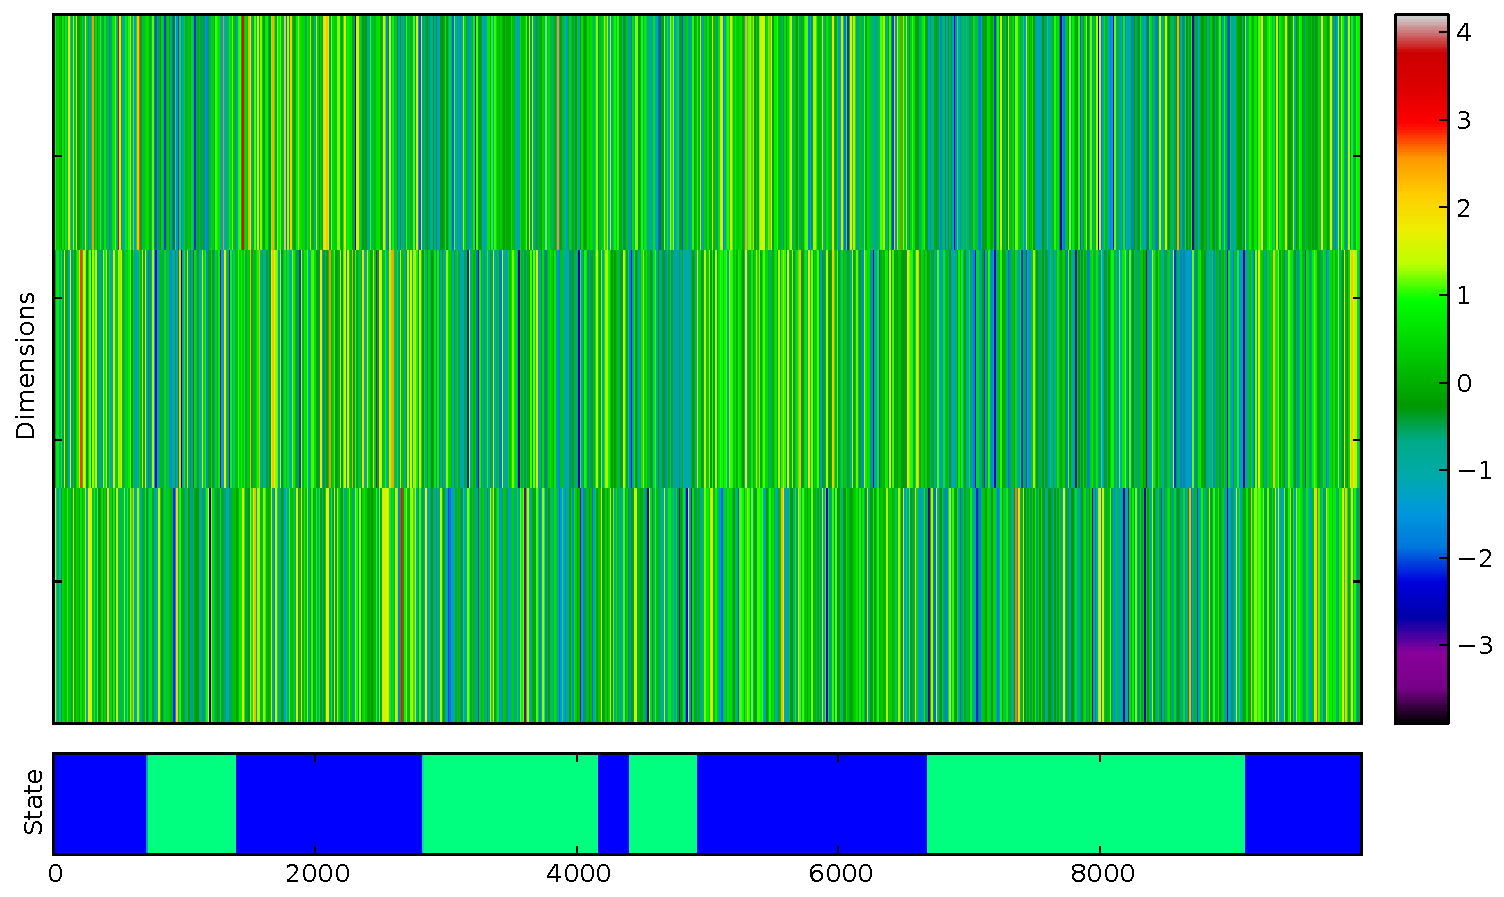
\includegraphics[width=1.\linewidth,
    height = 1.5in]{images/3D_synthetic_data_example.pdf}    
  \caption{\small{Simulated data example. Generated from two-state HMM with 3D
  Gaussian emissions and strong self-transitions.}}
  \label{fig:simulated}
\end{figure}
The second dataset is generated from real-world forty-five dimensional human accelerometer data, recorded for users performing five different activities, namely, playing basketball, rowing, jumping, ascending stairs and walking in a parking lot ~\cite{Altun:2010:CSC:1823245.1823314}. The data were recorded from a single subject using five Xsens MTx\texttrademark\ units attached to the torso, arms and legs. Each unit had nine sensors, which recorded accelerometer $(X, Y, Z)$ data, gyroscope $(X,Y,Z)$ data and magnetometer $(X,Y,Z)$ data, for a total of forty-five signals at each time point.

We generated one hundred multivariate times series from the underlying dataset,
with varying activities (latent states) and number of segments. To generate
these sets, we first uniformly chose the number of
segments, between two and twenty. Then, for each segment, we chose an activity
uniformly at random from among the five possible, and selected a uniformly
random segment length proportion. The selected number of corresponding time
points were extracted from the activity (keeping track of position in the
sequence, and modulo the length of the sequence), rescaled to zero mean and unit
variance, and appended to the output sequence. The final output sequence was
truncated to ten thousand time points, or discarded if the sequence contained
fewer than ten thousand points or fewer than two distinct activities.
Additionally, prospective time series were rejected and replaced if they caused
numerical instability issues for the algorithms tested, which occurred for some
time series with many (or extremely short) segments. This process produced
multivariate time series of fixed length, with varying number of segments,
activities and segment lengths. The process was repeated to generate one hundred
such time series of ten thousand time points each used in the quantitative
analysis described in Section~\ref{sec:quantitative}. An example of such
generated data sequences is shown in Figure~\ref{fig:accelerometer} and the
distribution of the time series according to number of activities and segments
is shown in Figure~\ref{fig:distribution}.

\begin{figure}[htbp]
  \centering
    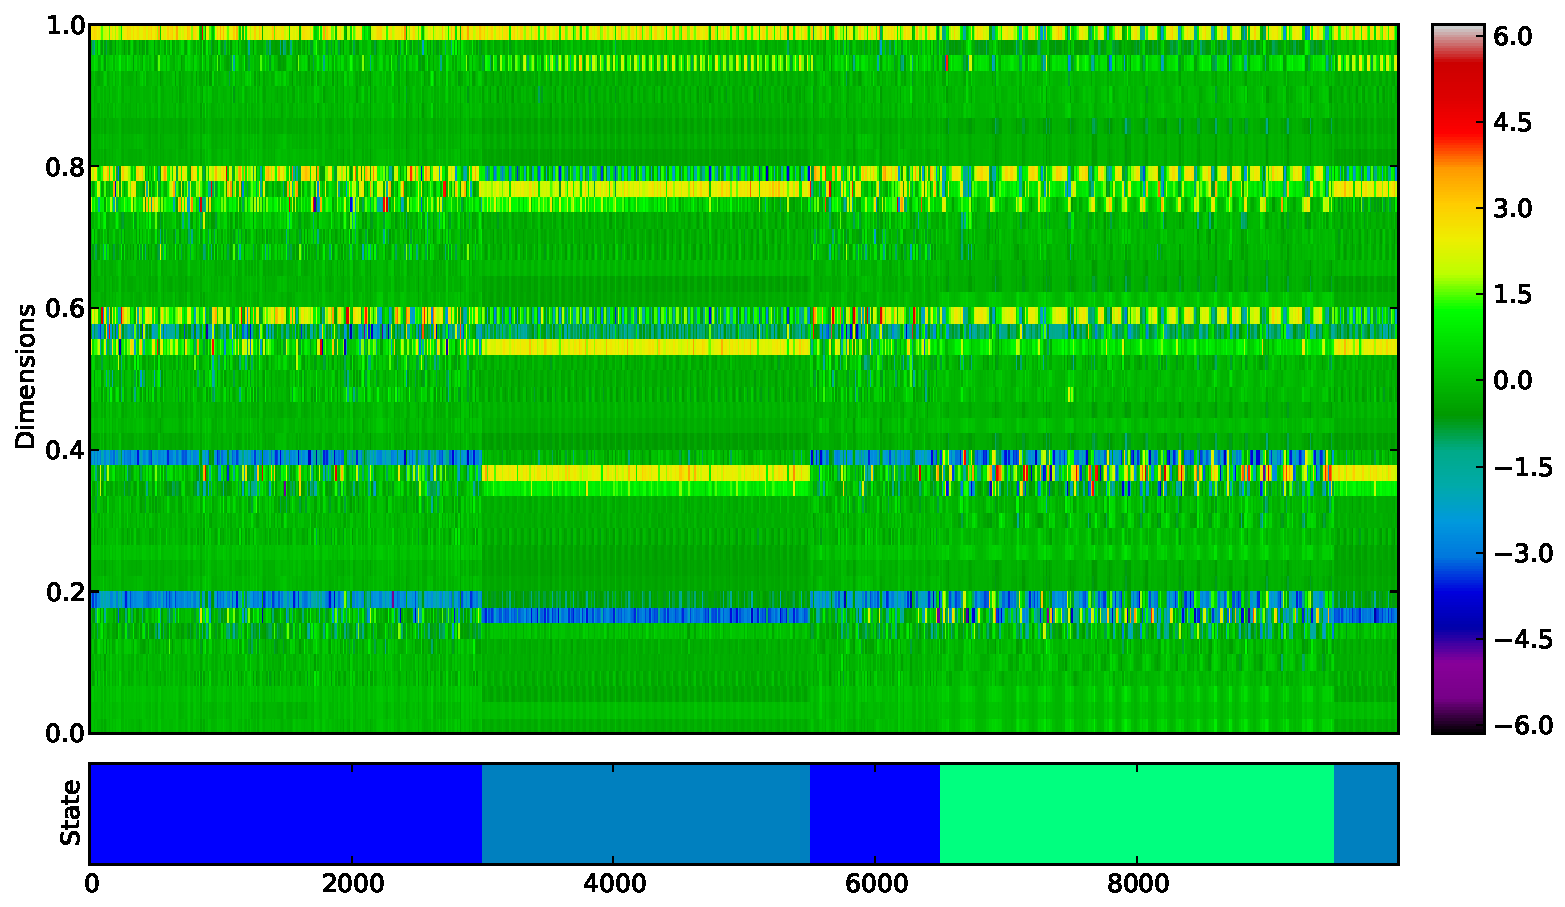
\includegraphics[width=1.\linewidth, height=1.5in]{images/accelerometer-data.pdf}
    \label{fig:accelerometer}
  \caption{\small{Human activities accelerometer data. Three state,
  45-dimensional.}}
\end{figure}

\begin{figure}[htbp]
  \centering
    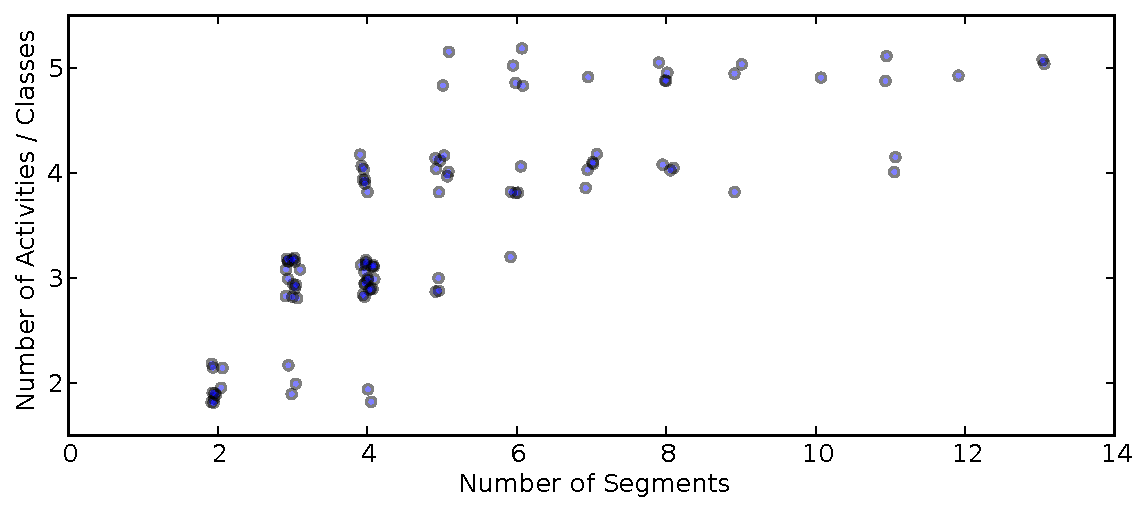
\includegraphics[width=1.\linewidth]{images/distribution_of_dataset_segments.pdf}
    \label{fig:distribution}
    \caption{\small{Distribution of Accelerometer Time Series Data.}}
\end{figure}

\subsection{Experimental Design and Evaluation Methods}

We compared performance of a standard $K$-state hidden Markov model with our
batch-learned regularized HMMs on the two datasets described in the previous
section. For the second dataset, we performed a quantitative analysis, treating
the task as a multi-class classification problem, and measured the minimum
zero-one loss under all possible permutations of output labels, to accommodate
the fact that the output labels of an HMM may be a permuted mapping of the true
labels. We measured the normalized variation of information~\cite{meila} between
the predicted state sequence and true state sequence, which is an information
metric capturing the distance between two
partitionings (clusterings) of a sequence. In addition to this, we considered
the ratio of predicted number of segments to true number of segments, which
gives us a sense of whether a method over- or under-segments data, and the
absolute segment number ratio (ASNR), which is defined as
$\text{ASNR} = \max(S_t, S_p)/\min(S_t, S_p)$, 
where $S_t$ is the true number of segments in the sequence and $S_p$ is the predicted number of segments. This value tells us how much a segmentation method diverges from the ground truth in terms of relative factor of segments. Lastly, we tracked the number of segments difference between the predicted segmentation and true segmentation and how many segmentations we done perfectly, giving the correct states at all correct positions.

To select parameters for the inertial regularized methods, we used the automated
parameter selection procedure discussed previously. To speed up evaluations, we only 
ran the automated parameter selection process on ten randomly drawn examples, averaged 
the final $\zeta$ parameter value, and used the fixed value for all evaluations. The 
final $\zeta$ parameters are shown in Tables~\ref{tab:results-synthetic} and \ref{tab:results-main}.

To evaluate the sticky HDP-HMM, we used the publicly available HDP-HMM toolbox for MATLAB,
with default settings for the priors~\cite{HDP-HMM-TOOLKIT}. The Gaussian emission model with normal
inverse Wishart (NIW) prior were used, and the truncation level $L$ for each
example was set to the true number of states, in fairness for comparing with the
HMM methods developed here, which are also given the true number of states. The
``stickiness'' $\kappa$ parameter was chosen in a data-driven manner by testing
values of $\kappa=0.001$, 0.01, 0.1, 1.0, 5.0, 10.0, 50.0, 100.0, 250.0, 500.0,
750.0 and 1000.0 for best performance over ten randomly selected examples each.
The mean performance of the 500th Gibbs sample of ten trials was then taken for
each parameter setting, and the best $\kappa$ was empirically chosen. For the
synthetic dataset, a final value of $\kappa=10$ was chosen by this method. For
the real human accelerometer data, a value of $\kappa=100.0$ provided the best
accuracy and relatively strong variation of information performance. These
values were used for evaluation on each entire dataset, respectively.

To evaluate the HDP-HMM, we performed five trials one each example in the test
dataset, measuring performance of the 1000th Gibbs sample for each trial. The
mean performance was then computed for the trials, and the average of all one
hundred test examples was recorded.
\begin{figure}[htbp]
  \centering
    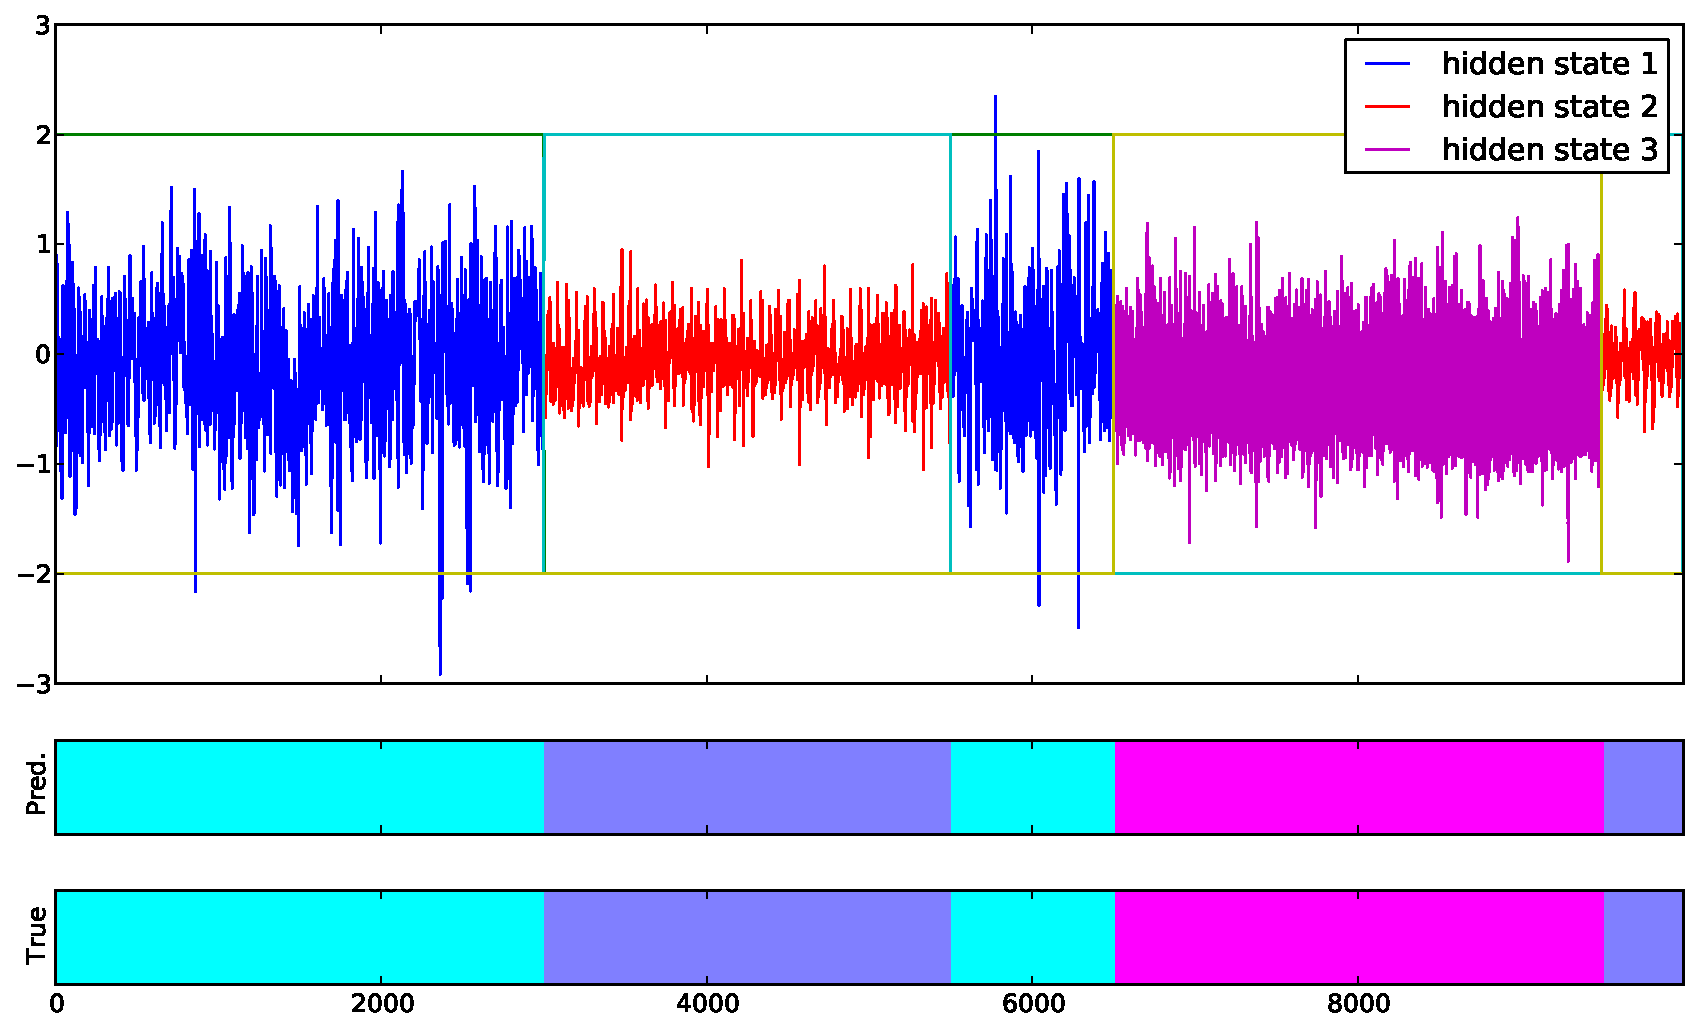
\includegraphics[width=0.8\linewidth, height=1.5in]{images/MAP_PARAM_FREE_results_hard_activity_long_1,97_3_states.pdf}    
    \caption{\small{Example segmentation of human activities accelerometer data
    using inertial (MAP) HMM}}
    \label{fig:real-results-MAP}
\end{figure}

\subsection{Synthetic Data Results}
\begin{table}[htbp]
\caption{\small{Results from quantitative evaluation on two-state, 3D synthetic
data.}} \resizebox{1.0\linewidth}{!}{
\begin{tabular}{|lrrrrrr|}
\hline
\textbf{Method}                   & \textbf{Acc.} & \textbf{SNR}  & \textbf{ASNR}     & \textbf{SND}  & \textbf{VOI}    & \textbf{Perfect}  \\ \hline
Sticky HDP-HMM ($\kappa = 10$)    & 0.85              & 0.59          & 3.50              & 2.79          & 0.56            & 0/100                          \\ 
Standard HMM                      & 0.87              & 172.20        & 172.20            & 765.91        & 0.62            & 0/100                          \\ 
MAP HMM ($\zeta = 2.28$)          & \textbf{0.99}     & \textbf{0.96} & \textbf{1.13}     & \textbf{0.51} & \textbf{0.07}   & \textbf{2/100}                 \\ 
Inertial PsO HMM ($\zeta = 8.19$) & \textbf{0.99}     & 0.87          & 1.43              & 1.15          & 0.14            & 1/100                          \\ \hline
\multicolumn{7}{l}{\begin{tabular}[c]{@{}l@{}}
    \vspace{0.05em}\\
    \textbf{Acc.} = Average Accuracy (value of 1.0 is best)\\ 
    \textbf{SNR} = Average Segment Number Ratio (value of 1.0 is best)\\ 
    \textbf{ASNR} = Average Absolute Segment Number Ratio (value of 1.0 is best)\\ 
    \textbf{SND} = Average Segment Number Difference (value of 0.0 is best)\\ 
    \textbf{VOI} = Average Normalized Variation of Information (value of 0.0 is best)\\ 
    \textbf{Perfect} = Total number of perfect/correct segmentations \end{tabular}} 
\end{tabular}
}
\label{tab:results-synthetic}
\end{table}
Results for the synthetic dataset are shown in
Table~\ref{tab:results-synthetic}. Overall, the MAP regularized HMM had the
strongest performance, with top scores on all metrics. The inertial
pseudo-observation HMM also had strong performance, with extremely high accuracy
and low variation of information. The standard HMM suffered from
over-segmentation of the data (as reflected in the high SNR, ASNR, and SND
scores), while the sticky HDP-HMM tended to under-segment the data. All methods
were able to achieve fairly high accuracy.

\subsection{Human Activities Accelerometer Data Results}\label{sec:quantitative}
\begin{table}[htbp]
\caption{Results from quantitative evaluation on multivariate human accelerometer data.}
\resizebox{1.0\linewidth}{!}{
\begin{tabular}{|lrrrrrr|}
\hline
\textbf{Method}                   & \textbf{Acc.} & \textbf{SNR}  & \textbf{ASNR}     & \textbf{SND}  & \textbf{VOI}    & \textbf{Perfect}  \\ \hline
Sticky HDP-HMM ($\kappa = 100$)   & 0.60              & 0.75          &  4.68             & 5.03          & 0.95            & 0/100                           \\ 
Standard HMM                      & 0.79              & 134.59        & 134.59            & 584.16        & 0.38            & 9/100                          \\ 
MAP HMM ($\zeta = 33.5$)          & \textbf{0.94}     & 1.28          & 1.43              & 2.62          & \textbf{0.14}   & \textbf{48/100}                 \\ 
Inertial PsO HMM ($\zeta = 49.0$) & \textbf{0.94}     & \textbf{1.03} & \textbf{1.29}     & \textbf{1.29} & 0.15            & \textbf{48/100}                 \\ \hline
\end{tabular}
}
\label{tab:results-main}
\end{table}

Results from the human accelerometer dataset are shown in
Table~\ref{tab:results-main}. Both the MAP HMM and inertial pseudo-observation
HMM achieved large gains in performance over the standard HMM model, with
average accuracy of 94\%. Furthermore, the number of segments was close to
correct on average, with a value near one in both the absolute and simple ratio
case. The average normalized variation of information was low for both the MAP and pseudo-observation methods.
Figure~\ref{fig:real-results-MAP} shows the segmentation results for the MAP
regularized HMM on a typical sequence, displaying a single dimension of the
multivariate time series for clarity. The regularized MAP HMM correctly segments
the time series, as can be seen from the congruence between the true and
predicted state transition histories (bottom of Figure~\ref{fig:real-results-MAP}).

In comparison, a standard hidden Markov model without inertial regularization
achieved accuracy of 79\%, but with average absolute SNR of
134.59 and average normalized variation of information value of $0.38$. On
average, the segmentations given by the standard HMM differed by $584.16$
segments, compared to the fewer than three segments difference between the
regularized HMMs and the ground truth sequences. Thus, the inertial
regularization produces drastic improvements for unsupervised segmentation of
human accelerometer activity data.

Even more striking was the improvement over the sticky HDP-HMM. The performance of that method was poor, with
normalized variation of information near 1 (i.e., no correlation between
the predicted and the true segment labels). The method tended to
under-segment the data, often collapsing to a single uniform output state, reflected in the SNR ratio 
having a value below one. Problems for this method may 
have resulted from the moderate dimensionality of the data, an issue suggested by Fox and Sudderth through
private correspondence. The sticky HDP-HMM suffers from slow mixing rates as the
dimensionality increases, and computation time explodes, being roughly cubic in
the dimension. As a result, the one hundred test examples took several days of
computation time to complete, whereas the inertial HMM methods took a few hours.

\section{Discussion}

Our results demonstrate the effectiveness of inertial regularization on HMMs for
time series segmentation. Although derived in two independent ways, the MAP
regularized and pseudo-observation inertial regularized HMM converge on a
similar maximum likelihood update equation, and thus, have similar performance.
Either version can be used for segmentation tasks, according to user preference.

The human activity task highlighted an issue with using standard HMMs for
segmentation of time series with infrequent state changes, namely,
over-segmentation. Incorporating regularization for state transitions provides a
simple solution to this problem. Since our methods rely on changing a single
update equation for a standard HMM learning method, they can be easily
incorporated into HMM learning libraries with minimal effort. This
ease-of-implementation gives a strong advantage over existing persistent-state
HMM methods, such as the sticky HDP-HMM framework.

While the sticky HDP-HMM performed moderately well on the low-dimensional
synthetic dataset, the default parameters produced poor performance on the
real-world accelerometer data. It remains possible that different settings of
hyperparameters may improve performance, but the cost of a combinatorial search
through hyperparameter space combined with the lengthy computation time of the
HDP-HMM method prohibited exhaustive exploration of the space. These results
show, at very least, a strong dependence on hyperparameter settings for
acceptable performance. In contrast, the inertial HMM methods presented here
make use of a simple heuristic for automatically selecting the strength
parameter $\zeta$, which resulted in excellent performance on both datasets
without the need for hand-tuning several hyperparameters. Although the sticky HDP-HMM 
has poor performance on the two segmentation tasks, there exist tasks for which the 
HDP-HMM method may be better suited (e.g., when the correct number of states is unknown).

\section{Related Work}

Hidden Markov models for sequential data have enjoyed a long history, gaining
popularity as a result of the widely influential tutorial by
Rabiner~\cite{rabiner1989tutorial}. Specific to the work presented here, the use
of regularization for HMM parameters received a general treatment
in~\cite{MAP1994}, for both transition and emission parameters. Our work details
a more specific version of the regularization, useful for state persistence.
Neukirchen and Rigoll~\cite{neukirchen1999controlling} studied the use of
regularization in HMMs for reducing parameter overfitting of emission
distributions due to insufficient training data, but without an emphasis on
inertial transitioning between states. Similarly,
Johnson~\cite{Johnson07whydoesnt} proposed using Dirichlet priors on multinomial
hidden Markov models as a means of enforcing sparse emission distributions.

Fox \emph{et al.}\ \cite{fox2011sticky} specifically developed a Bayesian sticky
HMM to provide inertial state persistence. They presented a method capable of
learning a hidden Markov model without specifying the number of states or
regularization strength beforehand, using a hierarchical Dirichlet process and
truncated Gibbs sampling. Their method requires a more complex approach to
learning the model and specification of several hyperparameters for the Bayesian priors 
along with a truncation limit. In contrast, our models only require the 
specification of two parameters, $K$ and $\zeta$, whereas the
sticky HDP-HMM requires analogous truncation level $L$ and $\kappa$ parameters
to be chosen, in addition to the hyperparameters on the model priors. 

\section{Conclusions}

To model changes in multivariate time series data, we derive two modified forms of hidden Markov model that effectively enforce state persistence. Although the methods derived here are simple, they perform well and are computationally tractable. We have shown that our inertial models are easily implemented, run efficiently, add almost no additional computation cost, and work well on data with moderate dimensions. Their simplicity is thus a feature and not a bug. 

We also presented a simple heuristic method for automated selection of the regularization-strength parameter. Our experiments on synthetic and real-world datasets show the effectiveness of our methods, giving large improvements in performance over standard HMMs and the sticky HDP-HMM.

The simplicity of our models pave the way for natural extensions, such as incremental parameter learning and changing the form of the class conditional emission distributions to incorporate internal dynamics. Such extensions are the focus of future work.

% \section{Acknowledgments}
% The authors would like to thank Emily Fox and Erik Sudderth for their discussions, feedback and assistance with use of the HDP-HMM toolbox.

\bibliographystyle{aaai}
\bibliography{references}

\end{document}
